\documentclass[12pt,fleqn,answers]{exam}
\usepackage{pifont}
\usepackage{dingbat}
\usepackage{amsmath,amssymb}
\usepackage{epsfig}
\usepackage{upgreek}
\usepackage[super]{nth}
\usepackage[colorlinks=true,linkcolor=black,anchorcolor=black,citecolor=black,filecolor=black,menucolor=black,runcolor=black,urlcolor=black]{hyperref}
\usepackage[letterpaper, margin=0.75in]{geometry}
\addpoints
\boxedpoints
\pointsinmargin
\pointname{pts}
\usepackage{tikz}
\usepackage{tkz-euclide}
\usetikzlibrary{shapes.geometric}
\usetikzlibrary{calc}
\usepackage[activate={true,nocompatibility},final,tracking=true,kerning=true,factor=1100,stretch=10,shrink=10]{microtype}
\usepackage[american]{babel}
\usepackage[T1]{fontenc}
\usepackage{fourier}
\usepackage{isomath}
\usepackage{upgreek,amsmath}
\usepackage{amssymb}
\usepackage{graphicx}

\newcommand{\dotprod}{\, {\scriptzcriptztyle\stackrel{\bullet}{{}}}\,}

\newcommand{\reals}{\mathbf{R}}
\newcommand{\lub}{\mathrm{lub}} 
\newcommand{\glb}{\mathrm{glb}} 
\newcommand{\complex}{\mathbf{C}}
\newcommand{\dom}{\mbox{dom}}
\newcommand{\range}{\mbox{range}}
\newcommand{\cover}{{\mathcal C}}
\newcommand{\integers}{\mathbf{Z}}
\newcommand{\vi}{\, \mathbf{i}}
\newcommand{\vj}{\, \mathbf{j}}
\newcommand{\vk}{\, \mathbf{k}}
\newcommand{\bi}{\, \mathbf{i}}
\newcommand{\bj}{\, \mathbf{j}}
\newcommand{\bk}{\, \mathbf{k}}
\DeclareMathOperator{\Arg}{\mathrm{Arg}}
\DeclareMathOperator{\Ln}{\mathrm{Ln}}
\newcommand{\imag}{\, \mathrm{i}}

\usepackage{graphicx}
\usepackage{color}
\shadedsolutions
\definecolor{SolutionColor}{rgb}{0.8,0.9,1}
\newcommand\AM{\textsc{am}}
\newcommand\PM{\textsc{pm}}
     
\newcommand{\quiz}{8}
\newcommand{\term}{Fall}
\newcommand{\due}{Wednesday 11 October at 13:15 \PM}
\newcommand{\class}{MATH 115}
\begin{document}
\large
\vspace{0.1in}
\noindent\makebox[3.0truein][l]{\textbf{\class}}
\textbf{Name:} \hrulefill \\
\noindent \makebox[3.0truein][l]{\textbf{In class work \quiz, \term \/ \the\year}}
\textbf{Row and Seat}:\hrulefill\\
\vspace{0.1in}


\noindent  In class work  \quiz\/  has questions 1 through  \numquestions \/ with a total of  \numpoints\/  points.   
Turn in your work at the end of class  \emph{on paper}. This assignment is due \emph{\due}.

\vspace{0.1in}


\begin{questions} 

    \question [1] The quantities $x$ and $y$ both depend on time $t$. Suppose that
    $ y = \tan(x)$. Further, suppose that at some moment, we have
    \[
         x = \frac{\uppi}{3} \mbox{ and } \frac{\mathrm{d} y}{\mathrm{d} t} = 42.    
    \]
    At this moment, find $y$ and $\frac{\mathrm{d} x}{\mathrm{d} t}$.

   \begin{solution} We have
   \[
      \frac{\mathrm{d}}{\mathrm{d}} \left[  y = \tan(x) \right] = \left[\frac{\mathrm{d} y}{\mathrm{d} t} =
      \sec(x)^2 \frac{\mathrm{d} x}{\mathrm{d} t} \right].
   \]
   Pasting in the data into the undifferentiated and differentiated equations, gives
   \[
      y = \tan \left(\frac{\uppi}{3}\right), \quad 42 =  \sec \left (\frac{\uppi}{3} \right)^2 \frac{\mathrm{d} x}{\mathrm{d} t}.   
   \]
   So
   \[
     y = \sqrt{3}  \mbox{ and }  \frac{\mathrm{d} x}{\mathrm{d} t}  = \frac{21}{2}.
   \]
   
   \end{solution}
    %\newpage

    \question [1] Assume a circular pancake. Buckwheat pancake batter is spreading out on a hot
    cast iron skillet.   At some moment, 
    the radius of the pancake is 4 inches and the rate of change of its 
    radius is $1/20$ inch per second.  At this moment, find the rate of 
    change of the area of the buckwheat pancake.

    \begin{solution} Let $A$ be the area. We have $A = \uppi r^2$. So
    \[
     \frac{\mathrm{d} A}{\mathrm{d} t} = 2 \uppi  r \frac{\mathrm{d} r}{\mathrm{d} t}
    \]
    Pasting in the data yields
    \[
     \frac{\mathrm{d} A}{\mathrm{d} t} = 2  \uppi \times  4 \times \frac{1}{20} = \frac{2 \uppi}{5} \mathrm{in}^2/\mathrm{sec}.
    \]
    
    \end{solution}
    \question For the labeled triangle shown below, assume that
    the quantities $A,B,C, \alpha, \beta,$ and $\gamma$ all depend on time $t$.

    \begin{center}
    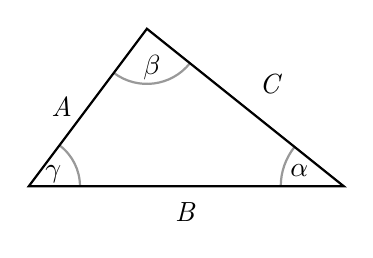
\begin{tikzpicture}[thick]
        \coordinate (O) at (0,0);
        \coordinate (A) at (4,0);
        \coordinate (B) at (1.5,2);
        \coordinate (C) at (1.5,0);
        \draw (O)--(A)--(B)--cycle;
       % \draw (C)--(B)--cycle;
        
        \tkzLabelSegment[below=2pt](O,A){\textit{B}}
        \tkzLabelSegment[left=2pt](O,B){\textit{A}}
        \tkzLabelSegment[above right=2pt](A,B){\textit{C}}
        %\tkzLabelSegment[right=2pt](C,B){\textit{h}}
        \tkzMarkAngle[fill= orange,size=0.65cm,%
        opacity=.4](A,O,B)
        \tkzLabelAngle[pos = 0.35](A,O,B){$\gamma$}
        
        \tkzMarkAngle[fill= orange,size=0.8cm,%
        opacity=.4](B,A,O)
        \tkzLabelAngle[pos = 0.6](B,A,O){$\alpha$}
        
        \tkzMarkAngle[fill= orange,size=0.7cm,%
        opacity=.4](O,B,A)
        \tkzLabelAngle[pos = 0.5](O,B,A){$\beta$}
        
        
        \end{tikzpicture}
    \end{center}
    At some moment, suppose
    \[
        A=1, \quad B=1, \quad  C=1, \quad 
        \frac{\mathrm{d} A}{\mathrm{d} t} = 8,
        \quad 
        \frac{\mathrm{d} B}{\mathrm{d} t} = 3,
        \quad 
        \frac{\mathrm{d} C}{\mathrm{d} t} = 2.
    \]

    \begin{parts}
     \part [1] At this moment, find 
     $\frac{\mathrm{d} \alpha}{\mathrm{d} t} = 2.$
     \part [1] At this moment, find the rate of change of
     the \emph{area} of the triangle.

    \end{parts}
    \begin{solution} Let's use the law of cosines:
    \[
      A^2 = B^2 + C^2 - 2 B C \cos(\alpha).
    \]
    Differentiating gives
    \[
     2 A A^\prime = 2 B B^\prime + 2 C C^\prime - 2 B^\prime C \cos(\alpha)
      - 2 B C^\prime \cos(\alpha) + 2 B C \sin(\alpha) \alpha^\prime.
    \]
   For the given data, the triangle is equilateral. So $\alpha= \uppi/3$. Pasting in this data and solving for 
   $ \alpha^\prime$ gives \( \alpha^\prime = \frac{11}{\sqrt{3}} $
     

   
   Also $\mathrm{Area} = \frac{1}{2} B C \sin(\alpha)$.  So
   \[
     \frac{\mathrm{d} \mathrm{Area}}{\mathrm{d} t} = \frac{1}{2} B^\prime  C \sin(\alpha) + 
     \frac{1}{2} B C^\prime \sin(\alpha) + \frac{1}{2} B  C \cos(\alpha) \alpha^\prime.     
   \]
   Pasting in the data gives
  \[
     \frac{d \mathrm{Area}}{\mathrm{d} t} = \frac{13}{2 \sqrt{3}}.  
   \]
          \end{solution}
\end{questions}


\end{document}

